
\subsection{Thermodynamical quantities}
\begin{frame}{Thermodynamical quantities}
	\centering
	Following, we are going to present physical quantities for both spin systems.\\[1em]
\end{frame}

%%%%%%%%%%%%%%%%%%%%%%%%%%%%%%%%%%%%%%%%
%%%%%%%%%%%%%%%%%%%%%%%%%%%%%%%%%%%%%%%%

\begin{frame}{Entropy}{\phantom{ }}
\only<+-2>{
Shannon entropy for a system is defined by 
\begin{equation}
	S = -\k \tilde{D}\sum_{\mathclap{s\,\in\,\text{states}}} \tilde{p}^{s} \ln \tilde{p}^{s},\label{eq:S_shann_orig}
\end{equation}
where $\tilde{D}$ is the total number of spins and $\tilde{p}^{s}$ are the probabilities of finding a spin on a state $s$.\\[1em]

\onslide<+->{%
In this case, we are going to use it as 
\begin{equation}
    S = - D\sum_{\mathclap{s\,\in\,\text{states}}} p^{s} \ln p^{s},\label{eq:S_shann}
\end{equation}
where $D$ is the total number of spins and $p^{s}$ are the probabilities of finding a spin on a state $s$.}
}
\only<+->{
\onslide<+->{%
\begin{itemize}
	\item For links:
\begin{equation}
    \label{eq:Sl}
	S_\ell  = - L \Big[ p_\ell^+\ln(p_\ell^+) + p_\ell^-\ln(p_\ell^-) \Big], 
\end{equation}
	\item For triangles:
\begin{equation}
    S_t = - C \Big[ p_t^+\ln(p_t^+) + p_t^-\ln(p_t^-) \Big], \label{eq:St}
\end{equation}}
\end{itemize}
\onslide<+>{%
Also, average entropies will be defined:
\begin{itemize}
	\item For links:
\begin{equation}
    \label{eq:sl}
	s_\ell  = \frac{S_\ell}{L}
\end{equation}
	\item For triangles:
\begin{equation}
	\label{eq:st}
    s_t = \frac{S_t}{C}
\end{equation}
\end{itemize}}}

\end{frame}
%%%%%%%%%%%%%%%%%%%%%%%%%%%%%%%%%%%%%%%%
%%%%%%%%%%%%%%%%%%%%%%%%%%%%%%%%%%%%%%%%

\begin{frame}{Results for link entropy}
\setlength\fboxsep{0pt}
\setlength\fboxrule{0pt}
\vspace{-2mm}
\begin{figure}[h]
 \centering
 \fbox{\adjincludegraphics[trim={{0.11\width} {0.135\height} {0.1\width} {0.184\height}},clip,height=0.8\textheight]{SE_plane}}
 \caption{\textbf{Link entropy} across different configurations on the configuration space. Plotted with $N=155$.}
 \label{fig:ps_sL}
\end{figure}
\end{frame}

\setlength\fboxsep{0pt}
\setlength\fboxrule{0pt}
\begin{frame}{Results for link entropy}
\vspace{-2mm}
\begin{figure}[h]
    \centering
    \fbox{%
    \adjincludegraphics[trim={{0.18\width} {0.135\height} {0.13\width} {0.184\height}},clip,height=0.8\textheight]{SE}}
    \caption{\textbf{Link entropy} plotted vertically against how many legislators have chosen each of two vote options. Plotted with $N=155.$}
    \label{fig:SL}
\end{figure}
\end{frame}

\begin{frame}{Results for link entropy}
	\makebox[\textwidth]{%
	\adjincludegraphics[trim={{0.18\width} {0.135\height} {0.13\width} {0.184\height}},clip,width=0.65\linewidth]{SE}
	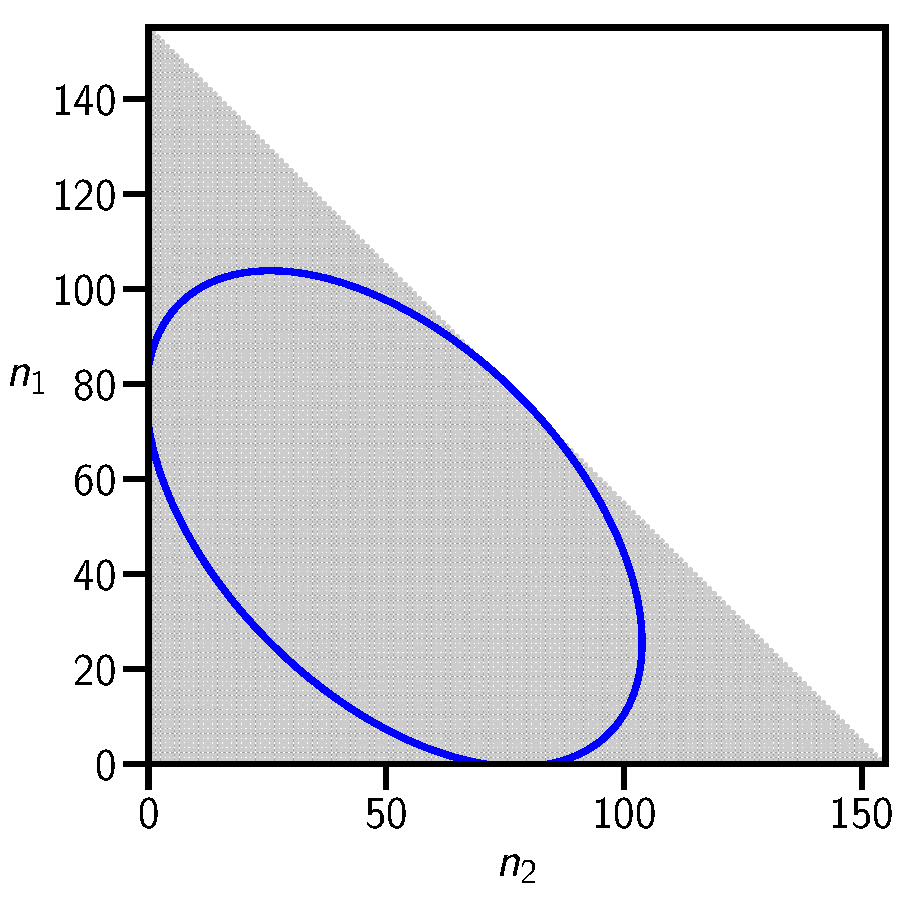
\includegraphics[width=0.47\linewidth]{elipse}
}
\captionof{figure}{\textbf{Link entropy} from \Cref{fig:SL} next to its maximum which was derived analytically.}
\end{frame}

\begin{frame}{Results for triangle entropy}
\setlength\fboxsep{0pt}
\setlength\fboxrule{0pt}
\vspace{-2mm}
\begin{figure}[h]
 \centering
 \fbox{\adjincludegraphics[trim={{0.11\width} {0.135\height} {0.10\width} {0.184\height}},clip,height=0.8\textheight]{ST_plane.pdf}}
 \caption{\textbf{Triangle entropy} across different configurations on the configuration space. Plotted with $N=155.$}
 \label{fig:ps_sT}
\end{figure}
\end{frame}



%%%%%%%%%%%%%%%%%%%%%%%%%%%%%%%%%%%%%%%%
%%%%%%%%%%%%%%%%%%%%%%%%%%%%%%%%%%%%%%%%

\begin{frame}{Magnetizations}{\phantom{ }}
	\onslide<+->{
		We define two types of magnetizations. For the links we will have 
		\begin{equation}
			M_\ell  = L^+ - L^-= \|\vec{n}\|^2  - \frac{N(N+1)}{2}, 
			\label{eq:Ml}
		\end{equation}
		and another for the triangles 
		\begin{equation}
			M_t = C^+ - C^- = \frac{1}{6} \left[ 2N -4 \|\vec{n}\|^{3}_{3} + 6N \|\vec{n}\|^{2} -3N^2 - N^3  \right]. 
			\label{eq:Mt}
		\end{equation}
	}
	\onslide<+->{
		We also define their average counter parts as 
		\begin{equation}
			m_\ell  = \frac{M_\ell}{L},
			\label{eq:ml}
		\end{equation}
		and
		\begin{equation}
			m_t = \frac{M_t}{C}.
			\label{eq:mt}
		\end{equation}
	}
\end{frame}

%%%%%%%%%%%%%%%%%%%%%%%%%%%%%%%%%%%%%%%%
%%%%%%%%%%%%%%%%%%%%%%%%%%%%%%%%%%%%%%%%

\begin{frame}{Results for link magnetizations}
\vspace{-2mm}
 \begin{figure}[h]
	 \setlength\fboxsep{0pt}
	 \setlength\fboxrule{0pt}
     \centering
     \fbox{\adjincludegraphics[trim={{0.10\width} {0.13\height} {0.1\width} {0.18\height}},clip,height=0.80\textheight]{results-figs/magE_plane}}%
     \caption{\textbf{Link magnetization} across different configurations on the configuration space. Plotted with $N=155.$}
     \label{fig:ps_magL}
 \end{figure}%
\end{frame}

\begin{frame}{Results for triangle magnetization}
\vspace{-2mm}
 \begin{figure}[h]
	 \setlength\fboxsep{0pt}
	 \setlength\fboxrule{0pt}
     \centering
     \fbox{\adjincludegraphics[trim={{0.10\width} {0.13\height} {0.1\width} {0.18\height}},clip,height=0.8\textheight]{magT_plane}}
     \caption{\textbf{Triangle magnetization} across different configurations on the configuration space. Plotted with $N=155.$}
     \label{fig:ps_magT}
 \end{figure}
\end{frame}


%%%%%%%%%%%%%%%%%%%%%%%%%%%%%%%%%%%
%%%%%%%%%%%%%%%%%%%%%%%%%%%%%%%%%%%

	
\begin{frame}{Hamiltonian}
	We define the energy for the system in such way it is minimal when everyone agrees with each other. 
\begin{itemize}
	\item All links would be positive
	\item All its triangles would be balanced 
\end{itemize}

For this, for a single triangle $t$ we have defined the energy function $h$ as
\begin{equation*}
    h(t) = - \sum_{\mathclap{\text{sides of $t$}}} \text{sign of the side} 
\end{equation*}
which is the negative sum of their sides. This would lead us to
\begin{center}
	\includesvg[width=0.7\columnwidth]{tri}
\end{center}
\vspace{-1mm}
\begin{equation*}
        h(+++) = -3,\qquad\quad
		h(---) = 3,\qquad\quad
		h(+--) = -1,
    \label{eq:h_types}
\end{equation*}
for each triangle type.\\[1em]
\end{frame}

\begin{frame}{Hamiltonian}
 Then, the energy for the whole system would be the sum of $h(t)$ for all triangles, or
 \begin{equation}
	H =	\sum_{\mathclap{t\in\text{triangles}}} h(t).
 \end{equation}
Since the network is fully-connected, each link belong to $(N-2)$ triangles. And since we are summing all of them, our Hamiltonian results 
\begin{equation}
	H = -(N-2)M_\ell.\label{eq:H_M}
\end{equation}
\end{frame}

%%%%%%%%%

\begin{frame}{Temperature}

Thermodynamical definition of temperature:
\begin{equation}
    \frac{1}{T} = \left( \frac{\partial S}{\partial U} \right)_{\,\mathclap{N}} \label{eq:T_def}
\end{equation}
where 
\begin{itemize}
	\item  $T$ is the temperature
	\item $S$ the entropy
	\item $N$ the number of particles
	\item and $U$ the internal energy.
\end{itemize}
In our case we would have

\begin{align}
    \frac{1}{T} &=  \frac{\partial S_\ell}{\partial H}  
\end{align}
\end{frame}

\begin{frame}{Temperature}
Expressing the link entropy as
\begin{equation*}
        S_\ell = - L\, \Biggr[\left(\frac{1+m_\ell}{2}\right) \ln\left(\frac{1+m_\ell}{2}\right) + \left(\frac{1-m_\ell}{2}\right)\ln \left(\frac{1-m_\ell}{2}\right)\Biggr]\label{eq:Sl_m},
\end{equation*}
we can solve for $\frac{1}{T}$. 
\begin{align*}
    \frac{1}{T} &= \frac{\p S_\ell}{\p m_\ell} \frac{\p m_\ell}{\p H}.
\end{align*}

After solving both partial derivatives we get 
\begin{equation}
	T = 2(N-2)\left[\ln \left(\frac{1+m_\ell}{1-m_\ell}\right) \right]^{-1}\label{eq:T_final}
\end{equation}

\end{frame}

%%%%%

\begin{frame}{Results for the temperature}
\vspace{-1mm}
\begin{figure}[h]
    \centering
    \fbox{\adjincludegraphics[trim={{0.13\width} {0.12\height} {0.11\width} {0.17\height}},clip,height=0.78\textheight]{Tps}}%
	\vspace{-1mm}
    \caption{\textbf{Temperature} on top of the configuration space. Plotted with $N=155$.}
    \label{fig:Tps}
\end{figure}
\end{frame}

\begin{frame}{Results for the temperature}
\vspace{-1mm}
\begin{figure}[h]
    \centering
    \fbox{\adjincludegraphics[trim={{0.16\width} {0.125\height} {0.17\width} {0.12\height}},clip,height=0.78\textheight]{Tpos-neg}}%
	\vspace{-1mm}
    \caption{Sign of temperature on top of configuration space. Plotted with $N=155.$}
    \label{fig:Tpos-neg}
\end{figure}
\end{frame}


%%%%%%%%%%%%%%%%%%%%%%%%%%%%%%%%%%%
%%%%%%%%%%%%%%%%%%%%%%%%%%%%%%%%%%%

\begin{frame}{Results for the temperature}{Temperature and energy}
	\setlength\fboxrule{0.5pt}
	\setlength\fboxsep{4pt}
\fbox{\begin{minipage}{0.5\textwidth}
		Let's recall that
	\begin{align*}
		M_\ell &= L\,m_\ell\\
		H &= -(N-2)M_{\ell}\\
		T &= 2(N-2)\left[\ln \left(\frac{1+m_\ell}{1-m_\ell}\right) \right]^{-1}
	\end{align*}
\end{minipage}}\\[1em]

	If we isolate $m_\ell$ from the temperature expression, we get that 	
\begin{equation}
    m_\ell = \tanh \left(\frac{N-2}{T}\right).\label{eq:ml_of_T}
\end{equation}
Now, joining it with the expressions for $H$ and $M_\ell$, it yield us that
\begin{align}
    H = -(N-2)L\tanh \left(\frac{N-2}{T}\right). \label{eq:H_of_T}
\end{align}
\end{frame}

\begin{frame}{Results for the temperature}{Temperature and energy}
	\begin{figure}[h]
	    \centering
		\includegraphics[height=0.65\textheight]{T_H}
	    \caption{Hamiltonian against temperature, from \cref{eq:H_of_T} with $N=155$. $H$ is not defined of for $T=0$, but in the plot it was considered as zero for visualization purposes.}
	    \label{fig:T_H_out}
	\end{figure}    
\end{frame}

%%%%%%%%%%%%%%%%%%%%%%%%%%%%%%%%%%
%%%%%%%%%%%%%%%%%%%%%%%%%%%%%%%%%%

